\documentclass[twoside]{book}

% Packages required by doxygen
\usepackage{fixltx2e}
\usepackage{calc}
\usepackage{doxygen}
\usepackage[export]{adjustbox} % also loads graphicx
\usepackage{graphicx}
\usepackage[utf8]{inputenc}
\usepackage{makeidx}
\usepackage{multicol}
\usepackage{multirow}
\PassOptionsToPackage{warn}{textcomp}
\usepackage{textcomp}
\usepackage[nointegrals]{wasysym}
\usepackage[table]{xcolor}

% Font selection
\usepackage[T1]{fontenc}
\usepackage[scaled=.90]{helvet}
\usepackage{courier}
\usepackage{amssymb}
\usepackage{sectsty}
\renewcommand{\familydefault}{\sfdefault}
\allsectionsfont{%
  \fontseries{bc}\selectfont%
  \color{darkgray}%
}
\renewcommand{\DoxyLabelFont}{%
  \fontseries{bc}\selectfont%
  \color{darkgray}%
}
\newcommand{\+}{\discretionary{\mbox{\scriptsize$\hookleftarrow$}}{}{}}

% Page & text layout
\usepackage{geometry}
\geometry{%
  a4paper,%
  top=2.5cm,%
  bottom=2.5cm,%
  left=2.5cm,%
  right=2.5cm%
}
\tolerance=750
\hfuzz=15pt
\hbadness=750
\setlength{\emergencystretch}{15pt}
\setlength{\parindent}{0cm}
\setlength{\parskip}{3ex plus 2ex minus 2ex}
\makeatletter
\renewcommand{\paragraph}{%
  \@startsection{paragraph}{4}{0ex}{-1.0ex}{1.0ex}{%
    \normalfont\normalsize\bfseries\SS@parafont%
  }%
}
\renewcommand{\subparagraph}{%
  \@startsection{subparagraph}{5}{0ex}{-1.0ex}{1.0ex}{%
    \normalfont\normalsize\bfseries\SS@subparafont%
  }%
}
\makeatother

% Headers & footers
\usepackage{fancyhdr}
\pagestyle{fancyplain}
\fancyhead[LE]{\fancyplain{}{\bfseries\thepage}}
\fancyhead[CE]{\fancyplain{}{}}
\fancyhead[RE]{\fancyplain{}{\bfseries\leftmark}}
\fancyhead[LO]{\fancyplain{}{\bfseries\rightmark}}
\fancyhead[CO]{\fancyplain{}{}}
\fancyhead[RO]{\fancyplain{}{\bfseries\thepage}}
\fancyfoot[LE]{\fancyplain{}{}}
\fancyfoot[CE]{\fancyplain{}{}}
\fancyfoot[RE]{\fancyplain{}{\bfseries\scriptsize Generated by Doxygen }}
\fancyfoot[LO]{\fancyplain{}{\bfseries\scriptsize Generated by Doxygen }}
\fancyfoot[CO]{\fancyplain{}{}}
\fancyfoot[RO]{\fancyplain{}{}}
\renewcommand{\footrulewidth}{0.4pt}
\renewcommand{\chaptermark}[1]{%
  \markboth{#1}{}%
}
\renewcommand{\sectionmark}[1]{%
  \markright{\thesection\ #1}%
}

% Indices & bibliography
\usepackage{natbib}
\usepackage[titles]{tocloft}
\setcounter{tocdepth}{3}
\setcounter{secnumdepth}{5}
\makeindex

% Hyperlinks (required, but should be loaded last)
\usepackage{ifpdf}
\ifpdf
  \usepackage[pdftex,pagebackref=true]{hyperref}
\else
  \usepackage[ps2pdf,pagebackref=true]{hyperref}
\fi
\hypersetup{%
  colorlinks=true,%
  linkcolor=blue,%
  citecolor=blue,%
  unicode%
}

% Custom commands
\newcommand{\clearemptydoublepage}{%
  \newpage{\pagestyle{empty}\cleardoublepage}%
}

\usepackage{caption}
\captionsetup{labelsep=space,justification=centering,font={bf},singlelinecheck=off,skip=4pt,position=top}

%===== C O N T E N T S =====

\begin{document}

% Titlepage & ToC
\hypersetup{pageanchor=false,
             bookmarksnumbered=true,
             pdfencoding=unicode
            }
\pagenumbering{roman}
\begin{titlepage}
\vspace*{7cm}
\begin{center}%
{\Large My Project }\\
\vspace*{1cm}
{\large Generated by Doxygen 1.8.11}\\
\end{center}
\end{titlepage}
\clearemptydoublepage
\tableofcontents
\clearemptydoublepage
\pagenumbering{arabic}
\hypersetup{pageanchor=true}

%--- Begin generated contents ---
\chapter{Class Index}
\section{Class List}
Here are the classes, structs, unions and interfaces with brief descriptions\+:\begin{DoxyCompactList}
\item\contentsline{section}{\hyperlink{class_motion_tracker}{Motion\+Tracker} }{\pageref{class_motion_tracker}}{}
\end{DoxyCompactList}

\chapter{File Index}
\section{File List}
Here is a list of all documented files with brief descriptions\+:\begin{DoxyCompactList}
\item\contentsline{section}{/home/viki/\+E\+N\+P\+M808\+X\+\_\+\+Midterm/app/\hyperlink{main_8cpp}{main.\+cpp} \\*This is the main file to run the Motion Tracker }{\pageref{main_8cpp}}{}
\end{DoxyCompactList}

\chapter{Class Documentation}
\hypertarget{class_motion_tracker}{}\section{Motion\+Tracker Class Reference}
\label{class_motion_tracker}\index{Motion\+Tracker@{Motion\+Tracker}}
\subsection*{Public Member Functions}
\begin{DoxyCompactItemize}
\item 
Video\+Capture \hyperlink{class_motion_tracker_aeeac24436c107964defb0da343573d37}{get\+Video} ()
\item 
Mat \hyperlink{class_motion_tracker_af94699e8524f6227ab4f25283c80a1a8}{Processing} (Video\+Capture, Mat, Mat)
\item 
void \hyperlink{class_motion_tracker_a69e04a4d0a7b623284ca74d1b094cabf}{tagging} (Rect object\+Bounding\+Rectangle, Mat \&camera\+Feed)
\item 
void \hyperlink{class_motion_tracker_acc3e04289a770c5d25e7e25278c873c7}{search\+For\+Motion} (Mat threshold\+Image, Mat \&camera\+Feed)
\item 
bool \hyperlink{class_motion_tracker_ad3869c9b786a88ed9793341cdf1432cb}{control\+Loop} (bool, bool)
\end{DoxyCompactItemize}
\subsection*{Protected Attributes}
\begin{DoxyCompactItemize}
\item 
int {\bfseries the\+Object} \mbox{[}2\mbox{]} = \{ 0,0 \}\hypertarget{class_motion_tracker_a68439780de998db60971232ebb6b3fdb}{}\label{class_motion_tracker_a68439780de998db60971232ebb6b3fdb}

\item 
Rect {\bfseries object\+Bounding\+Rectangle} = Rect(0, 0, 0, 0)\hypertarget{class_motion_tracker_a0661e19b606bca62523e9cdc6886b278}{}\label{class_motion_tracker_a0661e19b606bca62523e9cdc6886b278}

\item 
bool {\bfseries object\+Detected} = false\hypertarget{class_motion_tracker_a87d43478bd5d4293235a147d76d245df}{}\label{class_motion_tracker_a87d43478bd5d4293235a147d76d245df}

\item 
bool {\bfseries tracking\+Enabled} = false\hypertarget{class_motion_tracker_ad640d0c57f39113a6f214b58c9faf93e}{}\label{class_motion_tracker_ad640d0c57f39113a6f214b58c9faf93e}

\item 
bool {\bfseries pause} = false\hypertarget{class_motion_tracker_ae6a0d8ea864475f48aa7282725554749}{}\label{class_motion_tracker_ae6a0d8ea864475f48aa7282725554749}

\item 
Mat {\bfseries frame1}\hypertarget{class_motion_tracker_a1e7a0b2b0149ff4bdac58afa15cacf9e}{}\label{class_motion_tracker_a1e7a0b2b0149ff4bdac58afa15cacf9e}

\item 
Mat {\bfseries frame2}\hypertarget{class_motion_tracker_ab517bfdb4f65083195fc92e096143f69}{}\label{class_motion_tracker_ab517bfdb4f65083195fc92e096143f69}

\item 
Mat {\bfseries gray\+Image1}\hypertarget{class_motion_tracker_a4769c2bbfe3b96ebaa9e306bcb70cf5b}{}\label{class_motion_tracker_a4769c2bbfe3b96ebaa9e306bcb70cf5b}

\item 
Mat {\bfseries gray\+Image2}\hypertarget{class_motion_tracker_ac5d3a7852498f8b567254d7db5df5ae8}{}\label{class_motion_tracker_ac5d3a7852498f8b567254d7db5df5ae8}

\item 
Mat {\bfseries difference\+Image}\hypertarget{class_motion_tracker_aeb9d5fbadebbaf5908a650a530c24420}{}\label{class_motion_tracker_aeb9d5fbadebbaf5908a650a530c24420}

\item 
Mat {\bfseries threshold\+Image}\hypertarget{class_motion_tracker_ae065eedf0bd07e5bd5648bd9c570e84a}{}\label{class_motion_tracker_ae065eedf0bd07e5bd5648bd9c570e84a}

\end{DoxyCompactItemize}
\subsection*{Static Protected Attributes}
\begin{DoxyCompactItemize}
\item 
static const int {\bfseries S\+E\+N\+S\+I\+T\+I\+V\+I\+T\+Y\+\_\+\+V\+A\+L\+UE} = 20\hypertarget{class_motion_tracker_ae5573a13e28208c112527f2f39e6a66f}{}\label{class_motion_tracker_ae5573a13e28208c112527f2f39e6a66f}

\item 
static const int {\bfseries B\+L\+U\+R\+\_\+\+S\+I\+ZE} = 10\hypertarget{class_motion_tracker_a58397526b49648d305f7703787f31c20}{}\label{class_motion_tracker_a58397526b49648d305f7703787f31c20}

\end{DoxyCompactItemize}


\subsection{Member Function Documentation}
\index{Motion\+Tracker@{Motion\+Tracker}!control\+Loop@{control\+Loop}}
\index{control\+Loop@{control\+Loop}!Motion\+Tracker@{Motion\+Tracker}}
\subsubsection[{\texorpdfstring{control\+Loop(bool, bool)}{controlLoop(bool, bool)}}]{\setlength{\rightskip}{0pt plus 5cm}bool Motion\+Tracker\+::control\+Loop (
\begin{DoxyParamCaption}
\item[{bool}]{tracking\+Enabled, }
\item[{bool}]{pause}
\end{DoxyParamCaption}
)}\hypertarget{class_motion_tracker_ad3869c9b786a88ed9793341cdf1432cb}{}\label{class_motion_tracker_ad3869c9b786a88ed9793341cdf1432cb}
$<$ this 10ms delay is necessary for proper operation of this program if removed, frames will not have enough time to referesh and a blank image will appear.

$<$ \textquotesingle{}esc\textquotesingle{} key has been pressed, exit program.

$<$ \textquotesingle{}t\textquotesingle{} has been pressed. this will toggle tracking

$<$ \textquotesingle{}p\textquotesingle{} has been pressed. this will pause/resume the code.

$<$ stay in this loop until

$<$ change pause back to false \index{Motion\+Tracker@{Motion\+Tracker}!get\+Video@{get\+Video}}
\index{get\+Video@{get\+Video}!Motion\+Tracker@{Motion\+Tracker}}
\subsubsection[{\texorpdfstring{get\+Video()}{getVideo()}}]{\setlength{\rightskip}{0pt plus 5cm}Video\+Capture Motion\+Tracker\+::get\+Video (
\begin{DoxyParamCaption}
{}
\end{DoxyParamCaption}
)}\hypertarget{class_motion_tracker_aeeac24436c107964defb0da343573d37}{}\label{class_motion_tracker_aeeac24436c107964defb0da343573d37}
$<$ video capture object.

$<$ adding video file \index{Motion\+Tracker@{Motion\+Tracker}!Processing@{Processing}}
\index{Processing@{Processing}!Motion\+Tracker@{Motion\+Tracker}}
\subsubsection[{\texorpdfstring{Processing(\+Video\+Capture, Mat, Mat)}{Processing(VideoCapture, Mat, Mat)}}]{\setlength{\rightskip}{0pt plus 5cm}Mat Motion\+Tracker\+::\+Processing (
\begin{DoxyParamCaption}
\item[{Video\+Capture}]{capture, }
\item[{Mat}]{frame1, }
\item[{Mat}]{frame2}
\end{DoxyParamCaption}
)}\hypertarget{class_motion_tracker_af94699e8524f6227ab4f25283c80a1a8}{}\label{class_motion_tracker_af94699e8524f6227ab4f25283c80a1a8}
$<$ their grayscale images (needed for absdiff() function)

$<$ resulting difference image

$<$ thresholded difference image (for use in find\+Contours() function)

$<$ convert frame1 to gray scale for frame differencing

$<$ convert frame2 to gray scale for frame differencing

$<$ perform frame differencing with the sequential images. This will output an \char`\"{}intensity image\char`\"{} do not confuse this with a threshold image, we will need to perform thresholding afterwards.

$<$ threshold intensity image at a given sensitivity value

$<$ blur the image to get rid of the noise. This will output an intensity image

$<$ threshold again to obtain binary image from blur output \index{Motion\+Tracker@{Motion\+Tracker}!search\+For\+Motion@{search\+For\+Motion}}
\index{search\+For\+Motion@{search\+For\+Motion}!Motion\+Tracker@{Motion\+Tracker}}
\subsubsection[{\texorpdfstring{search\+For\+Motion(\+Mat threshold\+Image, Mat \&camera\+Feed)}{searchForMotion(Mat thresholdImage, Mat &cameraFeed)}}]{\setlength{\rightskip}{0pt plus 5cm}void Motion\+Tracker\+::search\+For\+Motion (
\begin{DoxyParamCaption}
\item[{Mat}]{threshold\+Image, }
\item[{Mat \&}]{camera\+Feed}
\end{DoxyParamCaption}
)}\hypertarget{class_motion_tracker_acc3e04289a770c5d25e7e25278c873c7}{}\label{class_motion_tracker_acc3e04289a770c5d25e7e25278c873c7}
$<$ notice how we use the \textquotesingle{}\&\textquotesingle{} operator for object\+Detected and camera\+Feed. This is because we wish to take the values passed into the function and manipulate them, rather than just working with a copy. eg. we draw to the camera\+Feed to be displayed in the main() function.

$<$ these two vectors needed for output of find\+Contours

$<$ find contours of filtered image using open\+CV find\+Contours function find\+Contours(temp,contours,hierarchy,\+C\+V\+\_\+\+R\+E\+T\+R\+\_\+\+C\+C\+O\+M\+P,\+C\+V\+\_\+\+C\+H\+A\+I\+N\+\_\+\+A\+P\+P\+R\+O\+X\+\_\+\+S\+I\+M\+P\+L\+E );// retrieves all contours

$<$ if contours vector is not empty, we have found some objects

$<$ the largest contour is found at the end of the contours vector we will simply assume that the biggest contour is the object we are looking for.

$<$ make a bounding rectangle around the largest contour then find its centroid this will be the object\textquotesingle{}s final estimated position. \index{Motion\+Tracker@{Motion\+Tracker}!tagging@{tagging}}
\index{tagging@{tagging}!Motion\+Tracker@{Motion\+Tracker}}
\subsubsection[{\texorpdfstring{tagging(\+Rect object\+Bounding\+Rectangle, Mat \&camera\+Feed)}{tagging(Rect objectBoundingRectangle, Mat &cameraFeed)}}]{\setlength{\rightskip}{0pt plus 5cm}void Motion\+Tracker\+::tagging (
\begin{DoxyParamCaption}
\item[{Rect}]{object\+Bounding\+Rectangle, }
\item[{Mat \&}]{camera\+Feed}
\end{DoxyParamCaption}
)}\hypertarget{class_motion_tracker_a69e04a4d0a7b623284ca74d1b094cabf}{}\label{class_motion_tracker_a69e04a4d0a7b623284ca74d1b094cabf}
$<$ update the objects positions by changing the \textquotesingle{}the\+Object\textquotesingle{} array values

$<$ make some temp x and y variables so we dont have to type out so much

$<$ draw some crosshairs around the object

$<$ write the position of the object to the screen 

The documentation for this class was generated from the following files\+:\begin{DoxyCompactItemize}
\item 
/home/viki/\+E\+N\+P\+M808\+X\+\_\+\+Midterm/include/\hyperlink{_motion_tracker_8h}{Motion\+Tracker.\+h}\item 
/home/viki/\+E\+N\+P\+M808\+X\+\_\+\+Midterm/include/\hyperlink{_motion_tracker_8cpp}{Motion\+Tracker.\+cpp}\end{DoxyCompactItemize}

\chapter{File Documentation}
\hypertarget{_motion_tracker_8cpp}{}\section{/home/viki/\+E\+N\+P\+M808\+X\+\_\+\+Midterm/include/\+Motion\+Tracker.cpp File Reference}
\label{_motion_tracker_8cpp}\index{/home/viki/\+E\+N\+P\+M808\+X\+\_\+\+Midterm/include/\+Motion\+Tracker.\+cpp@{/home/viki/\+E\+N\+P\+M808\+X\+\_\+\+Midterm/include/\+Motion\+Tracker.\+cpp}}


This is the file where all the variables and funtions are defined.  


{\ttfamily \#include \char`\"{}stdafx.\+h\char`\"{}}\\*
{\ttfamily \#include $<$opencv/highgui.\+h$>$}\\*
{\ttfamily \#include $<$iostream$>$}\\*
{\ttfamily \#include $<$stdlib.\+h$>$}\\*
{\ttfamily \#include \char`\"{}Motion\+Tracker.\+h\char`\"{}}\\*
Include dependency graph for Motion\+Tracker.\+cpp\+:
\nopagebreak
\begin{figure}[H]
\begin{center}
\leavevmode
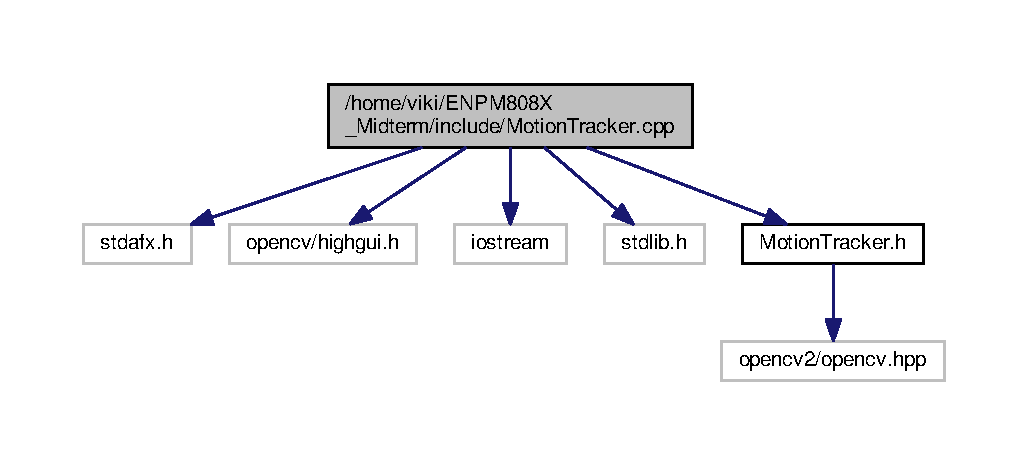
\includegraphics[width=350pt]{_motion_tracker_8cpp__incl}
\end{center}
\end{figure}


\subsection{Detailed Description}
This is the file where all the variables and funtions are defined. 

\begin{DoxyAuthor}{Author}
Akshay Bajaj 
\end{DoxyAuthor}
\begin{DoxyDate}{Date}
2017/10/14 
\end{DoxyDate}

\hypertarget{_motion_tracker_8h}{}\section{/home/viki/\+E\+N\+P\+M808\+X\+\_\+\+Midterm/include/\+Motion\+Tracker.h File Reference}
\label{_motion_tracker_8h}\index{/home/viki/\+E\+N\+P\+M808\+X\+\_\+\+Midterm/include/\+Motion\+Tracker.\+h@{/home/viki/\+E\+N\+P\+M808\+X\+\_\+\+Midterm/include/\+Motion\+Tracker.\+h}}


This is the file where all the variables and funtions are initialized under a class.  


{\ttfamily \#include \char`\"{}opencv2/opencv.\+hpp\char`\"{}}\\*
Include dependency graph for Motion\+Tracker.\+h\+:
\nopagebreak
\begin{figure}[H]
\begin{center}
\leavevmode
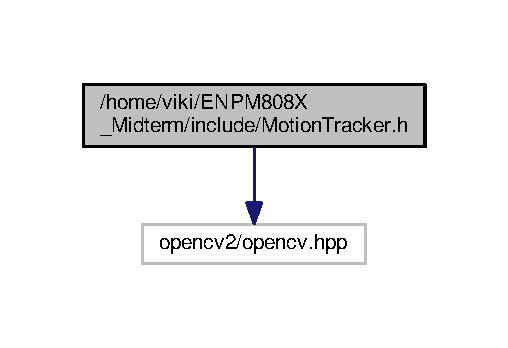
\includegraphics[width=244pt]{_motion_tracker_8h__incl}
\end{center}
\end{figure}
This graph shows which files directly or indirectly include this file\+:
\nopagebreak
\begin{figure}[H]
\begin{center}
\leavevmode
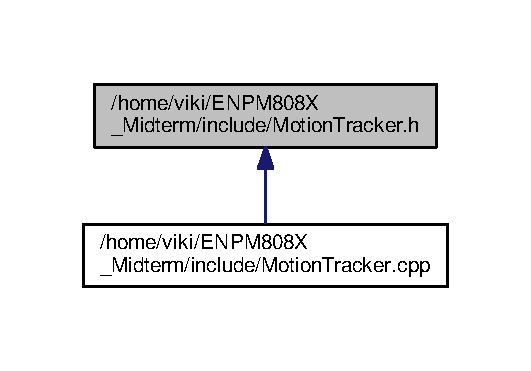
\includegraphics[width=255pt]{_motion_tracker_8h__dep__incl}
\end{center}
\end{figure}
\subsection*{Classes}
\begin{DoxyCompactItemize}
\item 
class \hyperlink{class_motion_tracker}{Motion\+Tracker}
\end{DoxyCompactItemize}


\subsection{Detailed Description}
This is the file where all the variables and funtions are initialized under a class. 

\begin{DoxyAuthor}{Author}
Akshay Bajaj 
\end{DoxyAuthor}
\begin{DoxyDate}{Date}
2017/10/10 
\end{DoxyDate}

%--- End generated contents ---

% Index
\backmatter
\newpage
\phantomsection
\clearemptydoublepage
\addcontentsline{toc}{chapter}{Index}
\printindex

\end{document}
